\documentclass[11pt,letterpaper]{article}
\usepackage{naaclhlt2013}
\usepackage{times}
\usepackage{latexsym}
\setlength\titlebox{3.5cm}    % Expanding the title-box

%%packaging we are adding
\usepackage{amsmath,amssymb}
\usepackage{amsthm}
\usepackage{ifthen}
\usepackage{graphicx}
\usepackage{stmaryrd}
\usepackage{enumitem}
\usepackage{multicol}
\usepackage{multirow}
\usepackage{CJKutf8}
\usepackage{algorithmic,algorithm,eqparbox,array}

\setlength\floatsep{1.25\baselineskip plus 3pt minus 2pt}
\setlength\textfloatsep{1\baselineskip plus 3pt minus 2pt}
\setlength\intextsep{1.25\baselineskip plus 3pt minus 2 pt}

%\newcommand\argmaxB[1]{
%    \underset{#1}{\operatorname{argmax}}
%}
\def\argmax{\underset{\mathbf{y} \in \mathrm{GEN}(\mathbf{x})}{\operatorname{argmax}}}
\def\argmaxb{\underset{\mathbf{y}}{\operatorname{argmax}}}
\def\argmaxk{\underset{\mathbf{k'}}{\operatorname{argmax}}}

%\underset{x}{\operatorname{argmax}}
%\input macros

\title{Two Knives Cut Better Than One: \\ Chinese Word Segmentation with Dual Decomposition} % too silly? too violent-sounding?
%what about, "Sharpening the Blade: Better..."
% or, "Sharpening the Knife" or hmm..
% or, "Two Knives are Sharper than One"
% or Scalpel instead of knife?
% or, "Cutting with Two Scalpels"? or Two Blades or Two Knives?

%\author{Author 1\\
%	    XYZ Company\\
%	    111 Anywhere Street\\
%	    Mytown, NY 10000, USA\\
%	    {\tt author1@xyz.org}
%	  \And
%	Author 2\\
%  	ABC University\\
%  	900 Main Street\\
%  	Ourcity, PQ, Canada A1A 1T2\\
%  {\tt author2@abc.ca}}

\begin{document}
\maketitle
\begin{CJK}{UTF8}{gbsn} % use CJK input

\begin{abstract}
There are two dominant approaches to Chinese word segmentation: word-based and character-based models, each with respective strengths. Prior work has shown that gains in segmentation performance can be achieved from combining these two types of models; however, past efforts have not provided a practical technique to allow mainstream adoption. We propose a method that effectively combines the strength of both segmentation schemes using an efficient dual-decomposition algorithm for joint inference. Our method is simple and easy to implement. Experiments on SIGHAN 2003 and 2005 evaluation datasets show that our method achieves the best reported results to date on 6 out of 7 datasets.
\end{abstract}

%%
%Word-based approaches are better at capturing longer context dependencies, and achieve higher segmentation consistency, whereas character-based approaches model the internal structures of words and can capture more out-of-vocabulary words. It is an intuitive idea to find methods to combine these approaches.  
\section{Introduction}

%First paragraph talks about why Chinese Word Segmentation is important.
Chinese text is written without delimiters between words; as a result, Chinese word segmentation (CWS) is an essential foundational step for many tasks in Chinese natural language processing. As demonstrated by \cite{Shi:2007:IJCAI,Bai:2008:IJCNLP,Chang:2008:ACL,Kummerfeld:2013:ACL}, the quality and consistency of segmentation has important downstream impacts on system performance in machine translation, POS tagging and parsing.

%Second paragraph talks about the challenges, specifically ambiguity and unknown words.
State-of-the-art performance in CWS is high, with F-scores in the upper 90s. %say this in a nicer way?
Still, challenges remain. Unknown words, also known as out-of-vocabulary (\textsc{oov}) words, lead to difficulties for word- or dictionary-based approaches.
Ambiguity can cause errors when the appropriate segmentation is determined contextually, such as 才能 (``talent") and 才 / 能 (``just able") \cite{Gao:2003:ACL}.

%Third paragraph: 
There are two primary classes of models: character-based \cite{Xue:2003:IJCLCLP,Tseng:2005:SIGHAN,Zhang:2006:HLT-NAACL,Wang:2010:COLING} and word-based \cite{Andrew:2006:EMNLP,Zhang:2007:ACL}, with corresponding advantages and disadvantages. \newcite{Sun:2010:COLING} details their theoretical distinctions: character-based approaches better model the internal compositional structure of words and are therefore more effective at inducing new out-of-vocabulary words; word-based approaches are better at reproducing the words of the training lexicon and can capture information from significantly larger contextual spans. Prior work has shown performance gains from combining these two types of models to exploit their respective strengths, but such approaches are often complex to implement and computationally expensive.
% too detailed?
%Due to the Markov assumption of the linear-chain CRFs that are commonly used in character-based segmentation the models typically only have information about the immediately neighboring characters, while word-based methods tend to capture information from significantly larger contextual spans.
%An additional advantage of word-segmenter is that they can explore larger context than character-based models (this is a little hard to explain without getting into the details of how these models work, maybe leave this piece till later; the basic idea is that character-based models -- i.e., linear-chain CRFs --- have very limited context due to Markov assumption, it typically only have direct information about the immediate neighboring characters, although information from longer-range context does flow because of the sentence-level normalization, its effect is much less direct. Word-based models in contrary directly captures the formation of entire words, say the previous word token has 3 characters, and the current word being considered has 3 characters, then a word-level bigram feature would capture context in neighboring 6 characters. 

In this work, we propose a simple and principled joint decoding method for combining character-based and word-based segmenters based on dual decomposition. This method has strong optimality guarantees and works very well empirically. It is easy to implement and does not require retraining of existing character- and word-based segmenters.
Experimental results on standard SIGHAN 2003 and 2005 bake-off evaluations show that our model outperforms the character and word baselines by a significant margin.
In particular, it improves \textsc{oov} recall rates and segmentation consistency, % this is now validated
and gives the best reported results to date on 6 out of 7 datasets. \label{sec:intro}
\section{Models for CWS}

In this section, we describe the character-based and word-based models we use as baselines, and review existing approaches to combine these models.

\subsection{Character-based Models}
In the most commonly used contemporary approach to character-based segmentation, first proposed by \cite{Xue:2003:IJCLCLP}, CWS is seen as a character sequence tagging task, where each character is tagged on whether it is at the beginning, middle, or end of a word. Conditional random fields (CRFs) are often used for this purpose (cite, cite, cite). In a CRF segmentation model, the probability of a label sequence is given by this equation:

%[add eq here]
% add defs of all the variables

Common linguistic features include character n-grams and morphological suffix/prefix features. Since these features capture information about the compositional properties of characters, they are likely to generalize well to unknown words.


\subsection{Word-based Models}

Initially word-based segmentation approaches employed simple heuristics like dictionary-lookup maximum matching \cite{Chen:1992:ACL}, contemporary approaches use machine learning techniques to solve an argmax problem of the form:

% add eq

The most successful such system reported to date is \cite{Zhang:2007:ACL}'s Perceptron-based model, which uses a search-based discriminative decoder to solve the ... %MQ add here?


%See \cite{Sun:2010:COLING} for a good description. We used the perceptron based model proposed by \cite{Zhang:2007:ACL}, give the equation of the perceptron, and describe the features. Point out how some of these features basically directly capture the training lexicon.
%
%\subsection{Relative Strength and Weakness}
%Char-based CRF models are better at generalizing over to OOV words (thus higher OOV recall).  (NOTE: 6 out of 8 datasets on test, CRF has better OOV recall, but we should defer to talk about this in the results section). But as a tradeoff, it generates more inconsistent segmentation, and creates lots of spurious words.
% The advantage of Word-based segmenters are that they are more consistent with the training lexicon, words seen in training lexicon are not likely to be segmented into many new ways; disadvantage is that it doesn't generalize well to OOV. Also exact inference is difficult, need to resolve to approximate decoding algorithms such as beam-searching.
% 

\subsection{Mixing Models} Since the two types of models described above have different strengths and make different kinds of errors, various mixing approaches have been proposed to combine them \cite{Wang:2006:SIGHAN,Lin:2009:CICLing,Sun:2009:HLT-NAACL,Sun:2010:COLING,Wang:2010:COLING}. 


\cite{Lin:2009:CICLing} and \cite{Wang:2006:SIGHAN} both incorporate a character-based Maxent local classifier model with a language model that captures more word-level context.
In order to bring in a bigram language model,  \shortcite{Lin:2009:CICLing} gave a heuristic decoding method that involves various forms of conditioning and back-off; \shortcite{Wang:2006:SIGHAN} gave a modified Viterbi algorithm with a complexity of $O(T^3)$. 

\cite{Sun:2009:HLT-NAACL} presented a latent-variable model which obtains good performance, but it is very complicated to implement and difficult to train. 
\cite{Sun:2009:HLT-NAACL} use a method most similar to this work in that they also directly combine two segmenters -- one char-based and one word-based. However, they do it through segmenter bagging, which requires training 50 or more individual segmenters and polling their results at test time. 

These mixing models perform well on standard datasets, but are not in wide use because of their high computational costs and difficulty of implementation. \label{sec:models}
%\section{Models for CWS}

In this section, we describe the character-based and word-based models we use as baselines, and review existing approaches to combine these models.

\subsection{Character-based Models}
In the most commonly used contemporary approach to character-based segmentation, first proposed by \cite{Xue:2003:IJCLCLP}, CWS is seen as a character sequence tagging task, where each character is tagged on whether it is at the beginning, middle, or end of a word. Conditional random fields (CRFs) are often used for this purpose (cite, cite, cite). In a CRF segmentation model, the probability of a label sequence is given by this equation:

%[add eq here]
% add defs of all the variables

Common linguistic features include character n-grams and morphological suffix/prefix features. Since these features capture information about the compositional properties of characters, they are likely to generalize well to unknown words.


\subsection{Word-based Models}

Initially word-based segmentation approaches employed simple heuristics like dictionary-lookup maximum matching \cite{Chen:1992:ACL}, contemporary approaches use machine learning techniques to solve an argmax problem of the form:

% add eq

The most successful such system reported to date is \cite{Zhang:2007:ACL}'s Perceptron-based model, which uses a search-based discriminative decoder to solve the ... %MQ add here?


%See \cite{Sun:2010:COLING} for a good description. We used the perceptron based model proposed by \cite{Zhang:2007:ACL}, give the equation of the perceptron, and describe the features. Point out how some of these features basically directly capture the training lexicon.
%
%\subsection{Relative Strength and Weakness}
%Char-based CRF models are better at generalizing over to OOV words (thus higher OOV recall).  (NOTE: 6 out of 8 datasets on test, CRF has better OOV recall, but we should defer to talk about this in the results section). But as a tradeoff, it generates more inconsistent segmentation, and creates lots of spurious words.
% The advantage of Word-based segmenters are that they are more consistent with the training lexicon, words seen in training lexicon are not likely to be segmented into many new ways; disadvantage is that it doesn't generalize well to OOV. Also exact inference is difficult, need to resolve to approximate decoding algorithms such as beam-searching.
% 

\subsection{Mixing Models} Since the two types of models described above have different strengths and make different kinds of errors, various mixing approaches have been proposed to combine them \cite{Wang:2006:SIGHAN,Lin:2009:CICLing,Sun:2009:HLT-NAACL,Sun:2010:COLING,Wang:2010:COLING}. 


\cite{Lin:2009:CICLing} and \cite{Wang:2006:SIGHAN} both incorporate a character-based Maxent local classifier model with a language model that captures more word-level context.
In order to bring in a bigram language model,  \shortcite{Lin:2009:CICLing} gave a heuristic decoding method that involves various forms of conditioning and back-off; \shortcite{Wang:2006:SIGHAN} gave a modified Viterbi algorithm with a complexity of $O(T^3)$. 

\cite{Sun:2009:HLT-NAACL} presented a latent-variable model which obtains good performance, but it is very complicated to implement and difficult to train. 
\cite{Sun:2009:HLT-NAACL} use a method most similar to this work in that they also directly combine two segmenters -- one char-based and one word-based. However, they do it through segmenter bagging, which requires training 50 or more individual segmenters and polling their results at test time. 

These mixing models perform well on standard datasets, but are not in wide use because of their high computational costs and difficulty of implementation. \label{sec:models}
%\section{Dual-Decomposition}

Dual decomposition offers a ideal framework for combining these two sources of signals without incurring high cost in model complexity (in contrast to \cite{Sun:2009:HLT-NAACL}) or decoding efficiency (in contrast to bagging in \cite{Wang:2006:SIGHAN,Sun:2010:COLING}).
DD has been successfully applied to similar situations where we want to combine local model with global models, for example, in dependency parsing \cite{Koo:2010:EMNLP}), bilingual sequence tagging \cite{Wang:2013:ACL} and word alignment \cite{}.  
Give a brief description of DD algorithm, focus on the intuition. See \cite{Wang:2013:ACL} and \cite{Denero:2011:ACL} for a good short introduction example.
Refer users to \cite{Rush:2012:JAIR} for a full tutorial on dual decomp.
The modification to Viterbi decoding is exactly the same as in \cite{Wang:2013:ACL} and \cite{Denero:2011:ACL}. The modification to the beam-search is similar, each time we extend a hypothesis with a new character, depending if the new character is appended to the last word or starting a new word, the corresponding DD penalty is factored into the score for the new hypothesis. 

 \label{sec:dual-decomp}
\section{Experiments}

Give URL for the Stanford CRF segmenter. The perceptron-based word segmenter is a re-implementation of \cite{Zhang:2007:ACL}.
For development data, we used:
Training: CTB section 1-270  400-931 1001-115;   Dev: CTB section 271-300.

Hyper-parameters tuned on the dev set.
Perceptron: 10 iterations of training. 
CRF: L2-regularization Sigma set to 3.
Dual-decomp: initial step size set to 0.1, 100 iterations. 

\subsection{Dataset}
Give description of the SIGHAN 2003 \cite{Sproat:2003:SIGHAN} and 2005 \cite{Emerson:2005:SIGHAN} bake-off datasets. 
List a table of the corpora names, size of training, testing, etc, similar to \cite{Sun:2010:COLING}.
 \label{sec:experiment}
\section{Results}

Reformat the table so it fits in a single column. 
The OOV rates should be moved out of this table and put in the data description tables in Experiment section Dataset subsection.

\begin{table*}
\centering
\begin{small}
\begin{tabular}{ l | l | c | c | c | c | c | c   }
\multicolumn{8}{c}{\large{SIGHAN 2005}} \\
%\cline{2-10}
%\hline
% &   \multicolumn{1}{|c}{Models} & \multicolumn{1}{c}{$\lambda$} & \multicolumn{1}{c|}{No. of experts} & {P} & {R} & {F$_1$}   & \multicolumn{1}{c}{P} & \multicolumn{1}{c}{R} & \multicolumn{1}{c}{F$_1$}   \\
\hline
    \multicolumn{2}{c}{}  &  \multicolumn{1}{c}{Recall} &  \multicolumn{1}{c}{Precision}  & \multicolumn{1}{c}{F$_1$}   &  \multicolumn{1}{c}{OOV} &   \multicolumn{1}{c|}{R$_{\mathrm{oov}}$}    &  \multicolumn{1}{c}{R$_{\mathrm{iv}}$}   \\ 
\hline
\multirow{4}{*}{AS} & SIGHAN winner      & 0.952 &  \textbf{0.951} & 0.952 &  0.043  &  0.696 &  0.963 \\
& CRF-Char                                                        & 0.952 &   0.936 & 0.944 & 0.043 &  0.589 & 0.969 \\
 & Perceptron-Word                                       & 0.958 & 0.950 & 0.954 & 0.043 & 0.695 & 0.970 \\ 
& Dual Decomp                                       & 0.959 & 0.949 & \textbf{0.954} & 0.043 & {0.677} & \textbf{0.972} \\
\hline

\multirow{4}{*}{PKU} &  SIGHAN winner       & \textbf{0.953}  &      0.946 &  0.950 & 0.058  &  0.636 &  \textbf{0.972} \\
& CRF-Char        & 0.946 &	0.953 & 0.949 &  0.058 &   0.778 &  0.956 \\
& Perceptron-Word  & 0.941 & 0.955	& 0.948 &  0.058 &  0.767 &  0.952 \\
& Dual Decomp  & 0.948 & \textbf{0.957} & \textbf{0.953} &  0.058 &  \textbf{0.787} &0.958 \\
\hline

\multirow{4}{*}{CITYU}  & SIGHAN winner       &  0.941 &  \textbf{0.946} & 0.943 & 0.074 & 0.698 & 0.961 \\
& CRF-Char       & 0.947 & 0.940 &  0.943 &  0.074 & \textbf{0.761} & 0.962 \\
& Perceptron-Word & 0.943 & 0.940 & 0.942 & 0.074 & 0.717  & 0.961  \\
& Dual Decomp & \textbf{0.950} & 0.944 & \textbf{0.947} & 0.074 & {0.753} & \textbf{0.965}  \\

\hline
\multirow{4}{*}{MSR} &  SIGHAN winner      & 0.962  & 0.966 &  0.964 &  0.026 &   0.717 &   0.968 \\
& CRF-Char        &  0.964 &   0.966 &  0.965 & 0.026 & 0.713 & 0.971 \\
& Perceptron-Word &  0.970 &  0.972 &  0.971 & 0.026 & 0.746 & 0.976 \\
& Dual Decomp & \textbf{0.973} &  \textbf{0.974} &  \textbf{0.974} & 0.026 & \textbf{0.760} & \textbf{0.979} \\
\hline
\multicolumn{8}{c}{\large{SIGHAN 2003}} \\
\hline

\multirow{4}{*}{AS}  &  SIGHAN winner     & 0.966     & 0.956 &  0.961 & 0.022 & 0.364 &  \textbf{0.980} \\
& CRF-Char    & 0.969 & 0.969 & 0.969 & 0.022 & 0.748 &  0.974 \\
& Perceptron-Word &  0.967 & 0.967 & 0.967 & 0.022 & 0.729  & 0.972 \\
& Dual Decomp & \textbf{0.970} & \textbf{0.971} & \textbf{0.971} & 0.022 & \textbf{0.775}  & 0.975 \\
\hline
\multirow{4}{*}{PKU}  &  SIGHAN winner        &   \textbf{0.962} &   0.940&  0.951 & 0.069 & 0.724 & \textbf{0.979} \\
& CRF-Char     &  0.954 & 0.952 & 0.953 & 0.069 & 0.803	 & 0.965 \\
& Perceptron-Word &  0.949 & 0.952 & 0.950 & 0.069 & 0.790  & 0.960 \\
& Dual Decomp &  0.954 & \textbf{0.954} & \textbf{0.954}	 & 0.069 & \textbf{0.806} & 0.965 \\
\hline
\multirow{4}{*}{CITYU}  &  SIGHAN winner   &  0.947   & 0.934  & 0.940 & 0.071  &  0.625  &  \textbf{0.972} \\
& CRF-Char       &  0.944 & 0.939 & 0.941 & 0.071  & 0.741   & 0.959 \\
& Perceptron-Word &  0.944 & 0.945 & 0.945 & 0.071  & 0.730  &  0.960 \\
& Dual Decomp &  \textbf{0.950} & \textbf{0.949} & \textbf{0.949} & 0.071 & \textbf{0.754} &  0.965 \\
\hline
\multirow{4}{*}{CTB}  &  SIGHAN winner  &  \textbf{0.886}  & 0.875 &  \textbf{0.881} & 0.181 & 0.644  & \textbf{0.927} \\
& CRF-Char       & 0.869 & 0.865 & 0.867 & 0.181 & 0.680  & 0.910 \\
& Perceptron-Word & 0.865 & 0.871 & 0.868 & 0.181 & 0.660 & 0.910 \\
& Dual Decomp  & 0.876 & \textbf{0.878} & 0.877 & 0.181 & \textbf{0.692} & 0.917  \\


\end{tabular} 
\caption{Results on SIGHAN 2005 and 2003 datasets. }\label{tbl:results}
\end{small}
\end{table*}

 \label{sec:results}
\section{Discussion and Error Analysis}

On the whole, dual decomposition produces state-of-the-art segmentations that are more accurate, more consistent, and more successful at inducing \textsc{oov} words than the baseline systems that it combines.
On the SIGHAN 2005 test set, over 99.1\% cases the DD algorithm converged within 100 iterations which gives optimality guarantee. 
In 77.4\% of the cases, DD converged in the first iteration. The number of iterations to convergence histogram is plotted in Figure~\ref{fig:histo}.

\paragraph{Error analysis}

%In the example below, dual decomposition output follows the incorrect segmentation of the character-based CRF in oversegmenting the compound "sea, land, and air." 

%%some errors where DD picks the wrong model:
%%gold: 有 亭台樓閣 流水
%%CRF: 亭台 樓閣  <-- DD
%%PCT: 亭台樓閣
%\begin{small}
%\begin{tabbing}
%\ \ \ \ \= \emph{Gloss}\ \ \ \ \= Large-scale / sea, land, and air / \\ 
%\> \> joint / military exercises\\
%\> \emph{Gold}\> 大规模 / 海陆空 / 联合 / 军演\\
%
%\> \emph{CRF}\> 大规模 / 海 / 陆空 / 联合 / 军演\\
%
%\> \emph{PCPT}\> 大规模 / 海陆空 / 联合 / 军演\\
%
%\> \emph{DD}\> 大规模 / 海 / 陆空 / 联合 / 军演\\
%\end{tabbing}
%\end{small}
In many cases the relative confidence of each model means that dual decomposition is capable of using information from both sources to generate a series of correct segmentations better than either baseline model alone. The example below shows a difficult-to-segment proper name comprised of common characters, which results in undersegmentation by the character-based CRF and oversegmentation by the word-based perceptron, but our method achieves the correct middle ground.

\begin{small}
\begin{tabbing}
\ \ \ \ \= \emph{Gloss}\ \ \ \ \= Tian Yage / 's / creations \\
\> \emph{Gold} \>   田雅各 / 的 / 创作 \\
\> \emph{CRF} \>  田雅各的 / 创作 \\
\> \emph{PCPT} \>  田雅 / 各 / 的 / 创作 \\
\> \emph{DD} \>  田雅各 / 的 / 创作 \\
\end{tabbing}
\end{small}

A powerful feature of the dual decomposition approach is that it can generate correct segmentation decisions in cases where a voting or product-of-experts model could not, since joint decoding allows the sharing of information at decoding time. In the following example, both baseline models miss the contextually clear use of the word 点心 (``sweets / snack food") and instead attach 点 to the prior word to produce the otherwise common compound 一点点 (``a little bit"); dual decomposition allows the model to generate the correct segmentation.
\begin{small}
\begin{tabbing}
\ \ \ \ \= \emph{English}\ \ \ \ \= Enjoy / a bit of / snack food / , ... \\
\> \emph{Gold} \>  享受 / 一点 / 点心 /  ,\\
\> \emph{CRF} \> 享受 / 一点点 / 心 / ,\\
\> \emph{PCPT} \> 享受 / 一点点 / 心 / , \\
\> \emph{DD} \>  享受 / 一点 / 点心 / ,\\
\end{tabbing}
\end{small}
We found more than 400 such surprisingly accurate instances in our dual decomposition output.

Finally, since dual decomposition is a method of joint decoding, it is liable to reproduce errors made by the constituent systems. 


\begin{figure}
\begin{center}
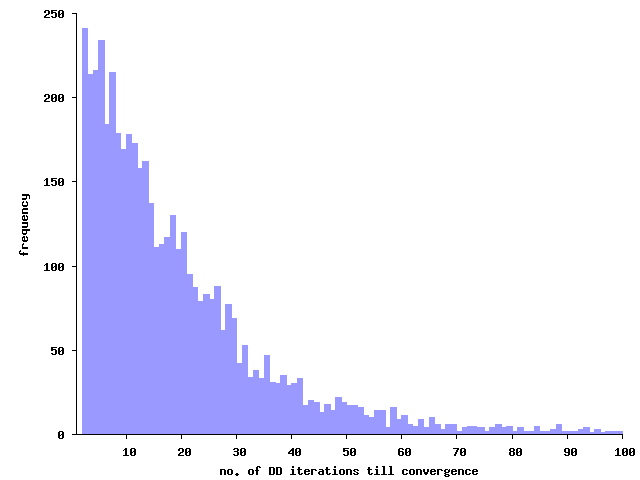
\includegraphics[width=\columnwidth]{histogram.png}
\caption{No. of iterations till DD convergence.}
\label{fig:histo}
\end{center}
\end{figure}



%
%gold: 在 李鄭屋邨 附近
%CRF: 在 李鄭屋邨 附近
%PCT: 在 李鄭屋 邨 附近   <-- DD
%
%gold: 麥 父 笑說
%CRF:  麥 父 笑說
%PCT: 麥父 笑說    <-- DD
%
%gold: 天氣 熱 時 冷氣 大 開     
%CRF: 天氣 熱 時 冷氣 大 開     
%PCT: 天氣 熱時 冷氣 大 開     <-- DD
 \label{sec:discussion}
%\section{Related Work}

\subsection{Character-based Models}
In the most commonly used contemporary approach to character-based segmentation, first proposed by \cite{Xue:2003:IJCLCLP}, CWS is seen as a character sequence tagging task, where each character is tagged on whether it is at the beginning, middle, or end of a word. Conditional random fields (CRFs) are often used for this purpose (cite, cite, cite). In a CRF segmentation model, the probability of a label sequence is given by this equation:

%[add eq here]
% add defs of all the variables

Common linguistic features include character n-grams and morphological suffix/prefix features. Since these features capture information about the compositional properties of characters, they are likely to generalize well to unknown words.


\subsection{Word-based Models}

Initially word-based segmentation approaches employed simple heuristics like dictionary-lookup maximum matching \cite{Chen:1992:ACL}, contemporary approaches use machine learning techniques to solve an argmax problem of the form:

% add eq



%See \cite{Sun:2010:COLING} for a good description. We used the perceptron based model proposed by \cite{Zhang:2007:ACL}, give the equation of the perceptron, and describe the features. Point out how some of these features basically directly capture the training lexicon.
%
%\subsection{Relative Strength and Weakness}
%Char-based CRF models are better at generalizing over to OOV words (thus higher OOV recall).  (NOTE: 6 out of 8 datasets on test, CRF has better OOV recall, but we should defer to talk about this in the results section). But as a tradeoff, it generates more inconsistent segmentation, and creates lots of spurious words.
% The advantage of Word-based segmenters are that they are more consistent with the training lexicon, words seen in training lexicon are not likely to be segmented into many new ways; disadvantage is that it doesn't generalize well to OOV. Also exact inference is difficult, need to resolve to approximate decoding algorithms such as beam-searching.
% 

\subsection{Mixing Models} Since the two types of models described above have different strengths and make different kinds of errors, various mixing approaches have been proposed to combine them \cite{Wang:2006:SIGHAN,Lin:2009:CICLing,Sun:2009:HLT-NAACL,Sun:2010:COLING,Wang:2010:COLING}. 


\cite{Lin:2009:CICLing} and \cite{Wang:2006:SIGHAN} both try to incorporate a character-based local classifier model (MaxEnt) with a language model that captures more word-level context.
In order to bring in bigram language model,  \shortcite{Lin:2009:CICLing} gave a heuristic decoding method that involves various conditioning and back-off; \shortcite{Wang:2006:SIGHAN} gave a modified Viterbi algorithm actually has complexity of $O(T^3)$. 

\cite{Sun:2009:HLT-NAACL} is the most similar in that they also try to directly combine two segmenters -- one char-based and one word-based. But they do it through segmenter bagging, which would require training up 50 or more individual segmenters and poll their results at test time, significantly increases training and testing effort, not practical.
\cite{Sun:2009:HLT-NAACL} presented a latent-variable model. very complicated, hard to train. our method is much simpler and works better than their method. \label{sec:relatedwork}
\section{Conclusion}

In this paper we presented an approach to Chinese word segmentation using dual decomposition for system combination. We demonstrated that this method allows for joint decoding of existing CWS systems that is more accurate and consistent than either system alone, and further achieves the best performance reported to date on standard datasets for the task.
Perhaps most importantly, our approach is straightforward to implement and does not require retraining of the underlying segmentation models used. This suggests its potential for broader applicability in real-world settings than existing approaches to combining character-based and word-based models for Chinese word segmentation. \label{sec:conclusion}


\bibliographystyle{naaclhlt2013}
\bibliography{emnlp_cws}
\end{CJK}
\end{document}
